\documentclass[10pt]{beamer}

% Configuration {{{
\usepackage[utf8]{inputenc}
\usepackage[T2A]{fontenc} % T1 for English
\usepackage[english, russian]{babel}

\usepackage{mathtools}
\usepackage{graphicx}
\usepackage{tikz}
\usepackage[multidot]{grffile}
\usepackage[labelsep=period]{caption}
\usepackage{multirow}

\setbeamertemplate{caption}[numbered]
\setbeamertemplate{navigation symbols}{}
\usefonttheme[onlymath]{serif}
\usepackage{DejaVuSansCondensed} % helvet for English
\usetheme{Madrid}

\linespread{1.2}

\usepackage{definitions}

\def\bottomleft#1#2{\phantom{#1}\hfill#2\hfill#1}
% }}}

% Title and other {{{
\title[Изучение многочастичных распадов $\Lb$]{
  Изучение многочастичных распадов прелестных барионов~$\Lb$
  в~эксперименте LHCb на~Большом адронном коллайдере
}
\author[Керим Гусейнов]{
  Керим Гусейнов
}
\institute[МГУ]{
  МГУ им. М.\,В.~Ломоносова
  \\ Физический факультет
  \\ Кафедра общей ядерной физики
}
\date{Ломоносов 2023, 11 апреля}

% }}}

\begin{document}

\frame[plain]{\titlepage}

\begin{frame}[label=introduction]%{{{
  \frametitle{Введение: распады прелестных барионов}

  \parbox{.55\linewidth}{
    \begin{itemize}
      \item Проверка непертурбативных подходов в~КХД,
      \item Большое высвобождение энергии, а~значит,
        богатая резонансная структура.
    \end{itemize}
    
    \vfill

    Переход $b \to c$ на~кварковом уровне:
    \begin{itemize}
      \item очарованный барион или $D$-мезон и~протон в~конечном 
        состоянии: адронизация $c$-кварка,
      %\item очарованный кварк адронизуется в~барион или мезон
      %  в~конечном состоянии,
      %\item очарованный адрон и~барион в~конечном состоянии
      %  ({\color{red} $c$-барион} или $D$-мезон + протон),
      \item изучение как очарованных мезонов, так и~барионов,
      \item разрешенный ККМ переход -- большая статистика событий.
    \end{itemize}
  } \parbox{.44\linewidth}{
    \centering
    %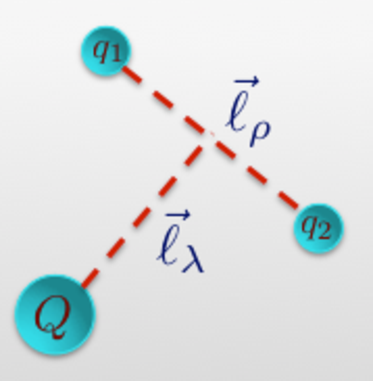
\includegraphics[width=.8\linewidth]{figures/hqet-quark-diquark}
    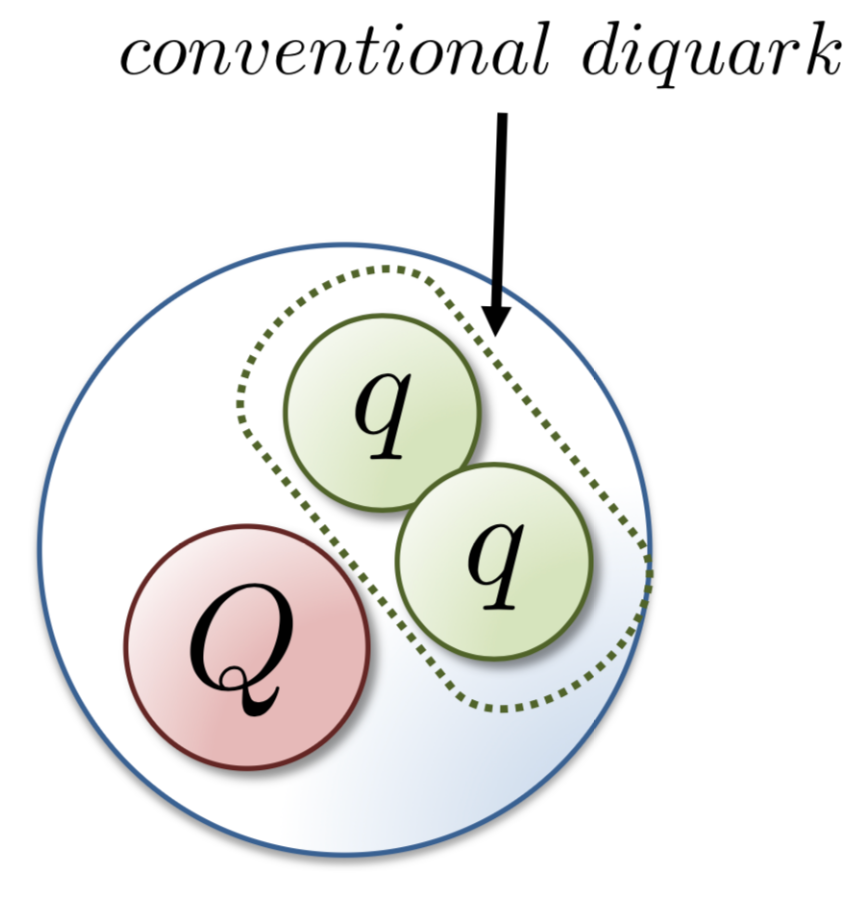
\includegraphics[height=.4\textheight]{figures/heavy-baryon-Qqq}
    \vfill
    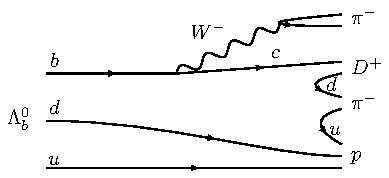
\includegraphics[width=\linewidth]{figures/diagram-lb2dppipi-bold}
    %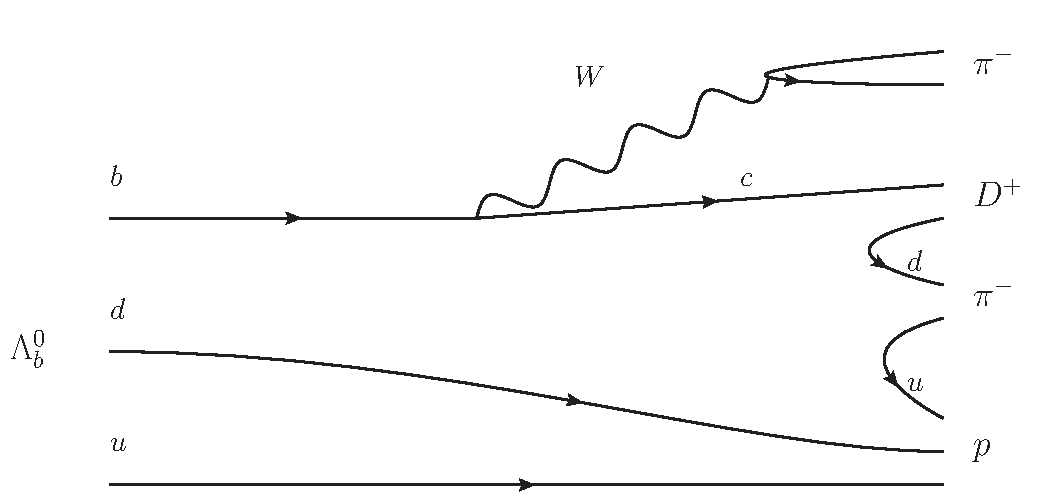
\includegraphics[width=\linewidth]{figures/diagram-lb2dppipi}
  }
  \vfill \centering Примеры:
  \hspace{2ex} $\Lb\to\Dp\p\pim\pim$,
  \hspace{2ex} $\Lb\to\Lc\pip\pim\pim$.
\end{frame}%}}}

\begin{frame}[label=resonances]%{{{
  \frametitle{Известные очарованные барионные резонансы}
  \centering
  \bottomleft{[PDG]}{
    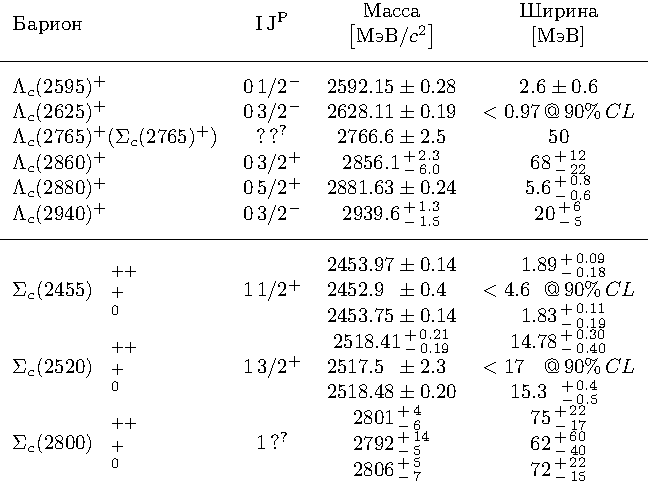
\includegraphics[width=.8\linewidth]{figures/resonances-table}
  }
\end{frame}%}}}

\begin{frame}[label=measurements-overview]%{{{
  \frametitle{Существующие измерения очарованных барионов}
  \centering
  \parbox{.41\linewidth}{ \centering
    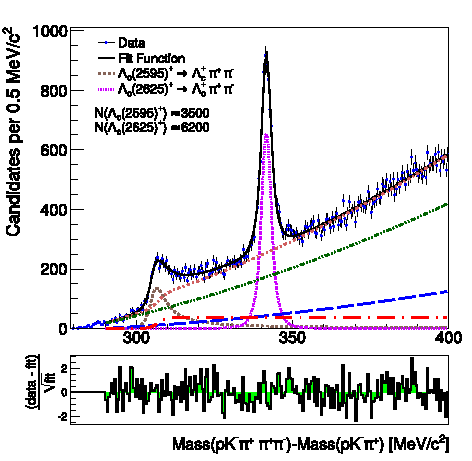
\includegraphics[width=.7\linewidth]{figures/src/lc2595-2625-cdf}
    \rotatebox{90}{$\LcI$, $\LcII$}
    \rotatebox{90}{[1106.5995] CDF}
  }
  \parbox{.58\linewidth}{ \centering
    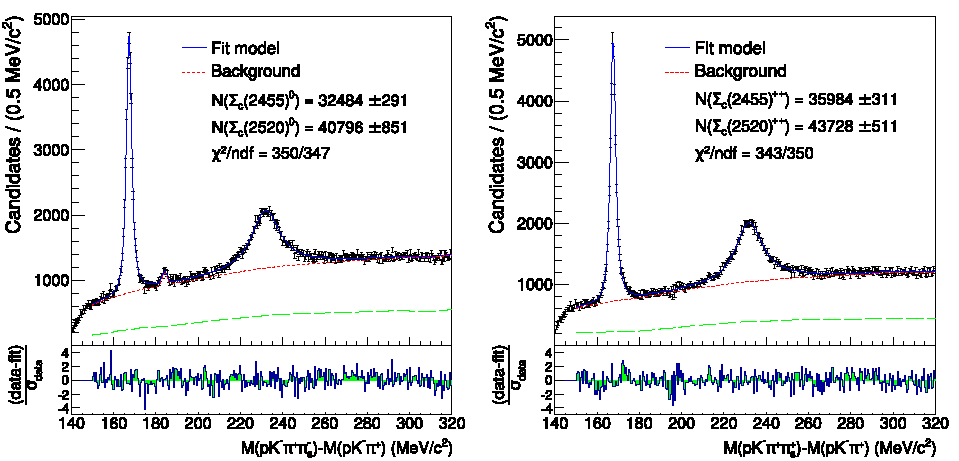
\includegraphics[width=.8\linewidth]{figures/src/sc2455-2520-belle}
    \rotatebox{90}{$\ScI$, $\ScII$}
    \rotatebox{90}{[1404.5389] Belle}
  }
  \vfill
  \parbox{.45\linewidth}{ \centering
    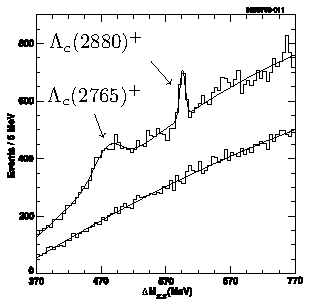
\includegraphics[width=.7\linewidth]{figures/lc2765-2880-cleo-mod}
    \rotatebox{90}{$\LcIIIother$, $\LcIII$}
    \rotatebox{90}{[hep-ex/0010080] CLEO}
  }
  \parbox{.45\linewidth}{ \centering
    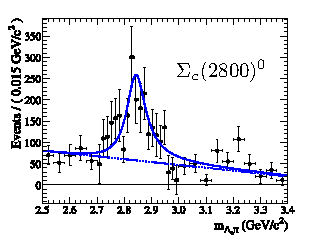
\includegraphics[width=.8\linewidth]{figures/sc2800-babar-mod}
    \rotatebox{90}{$\ScIIIz$}
    \rotatebox{90}{[0807.4974] BaBar}
  }
  %\parbox{.45\linewidth}{ \centering
  %  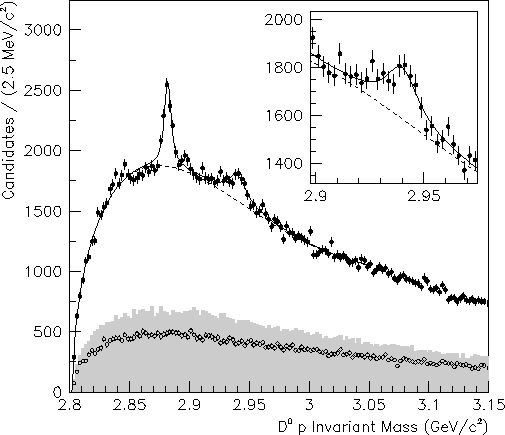
\includegraphics[width=.7\linewidth]{figures/src/lc2880-babar}
  %  \rotatebox{90}{$\LcIII$, BaBar}
  %  \rotatebox{90}{[hep-ex/0603052]}
  %}
  %\parbox{.45\linewidth}{ \centering
  %  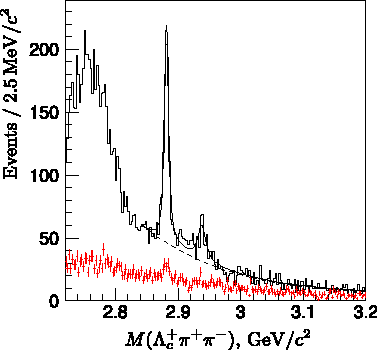
\includegraphics[width=.7\linewidth]{figures/src/lc2880-belle}
  %  \rotatebox{90}{$\LcIII$, Belle}
  %  \rotatebox{90}{[hep-ex/0608043]}
  %}
  % CLEO, Belle (старое и новое), BaBar, CDF
\end{frame}%}}}

\begin{frame}[label=lhcb]%{{{
  \frametitle{Детектор LHCb}
  \centering
  %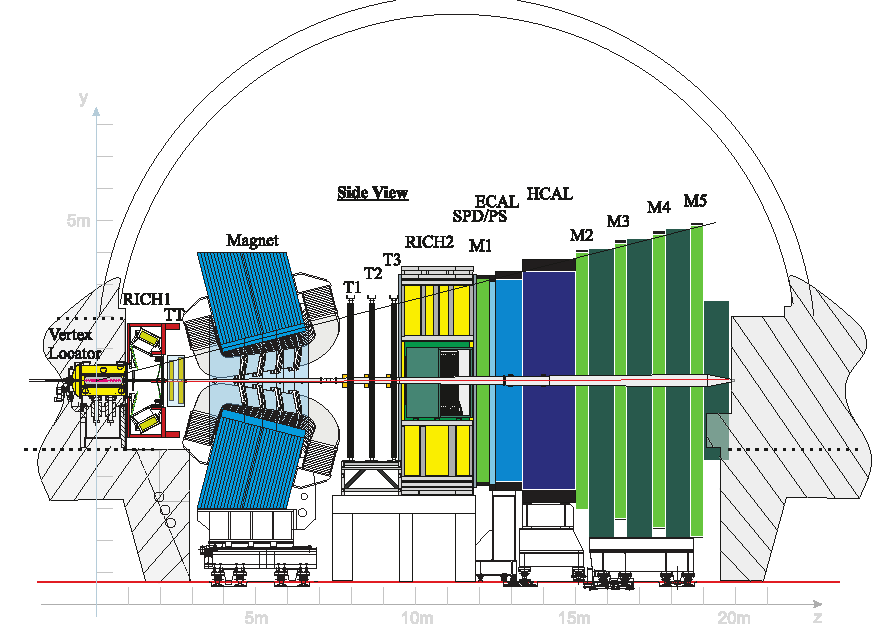
\includegraphics[width=.8\linewidth]{figures/lhcb-detector}
  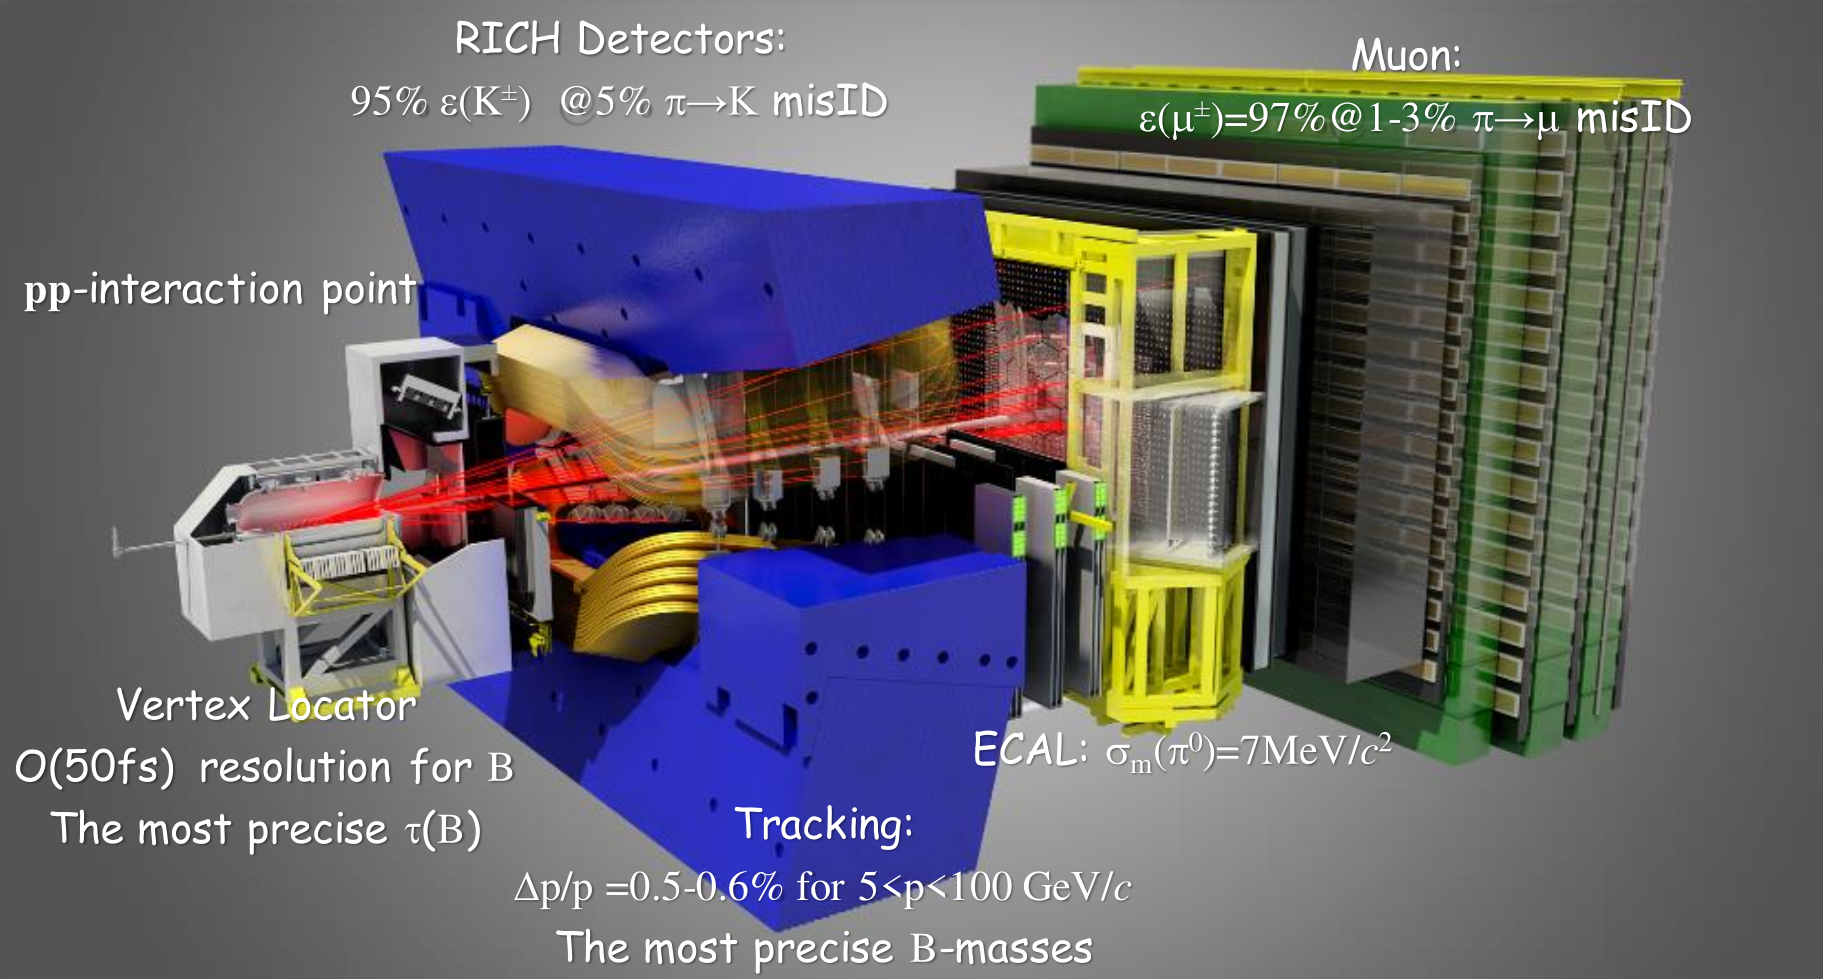
\includegraphics[height=.7\textheight]{figures/lhcb-detector-captions}
  \vfill [JINST \textbf{3} S08005]
\end{frame}%}}}

\begin{frame}[label=old-ana]%{{{
  \frametitle{$\Lb\to\Doptstarp\p\pim\pim$ и $\Lb\to\Lc3\pi$, Run 1 (2011--2012)}
  \centering
  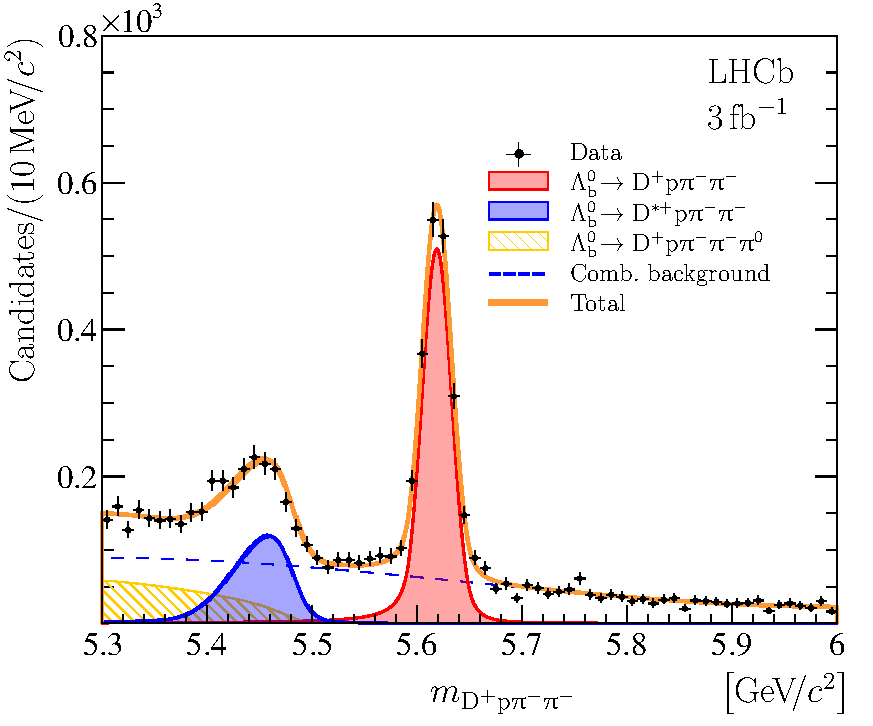
\includegraphics[width=.49\linewidth]{figures/fit-dppipi-run1}
  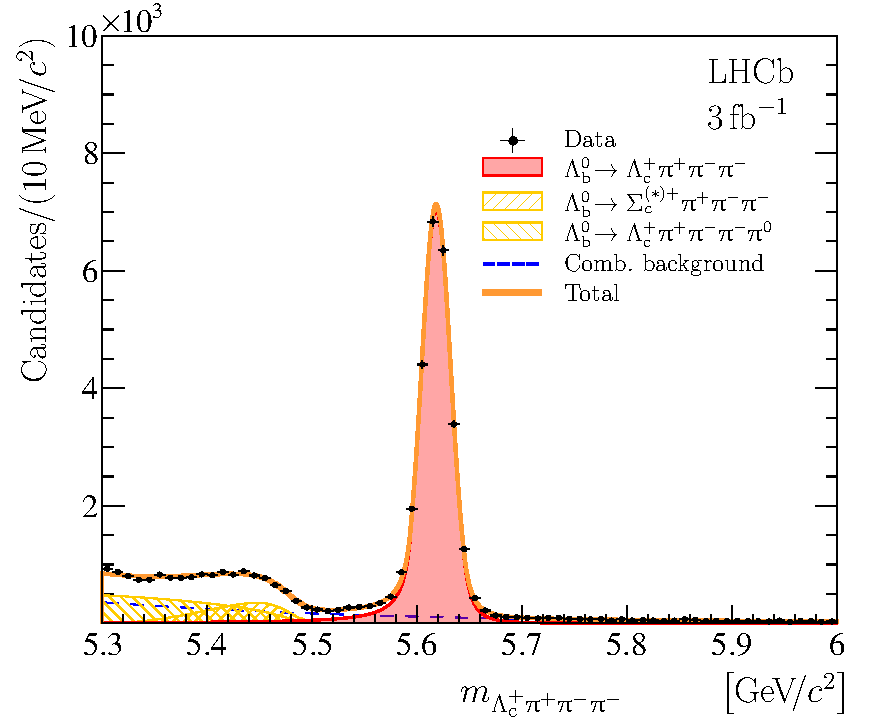
\includegraphics[width=.49\linewidth]{figures/fit-lc3pi-run1}
  \vfill
  \parbox{.49\linewidth}{\centering 2000 событий}
  \parbox{.49\linewidth}{\centering 26\,000 событий}
  \vfill \vfill
  [JHEP 03 (2022) 153]
\end{frame}%}}}

\begin{frame}[label=reweighting-spectra]%{{{
  \frametitle{Спектры $\Lc\pip\pim$, $\Lc\pim$, $\Lc\pip$ Run~1}
  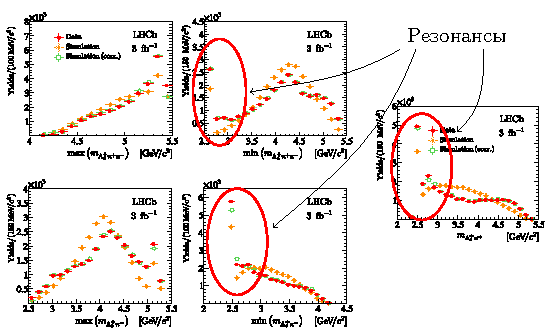
\includegraphics[width=\linewidth]{figures/reweighting-resonances}
  %\parbox{.66\linewidth}{
  %  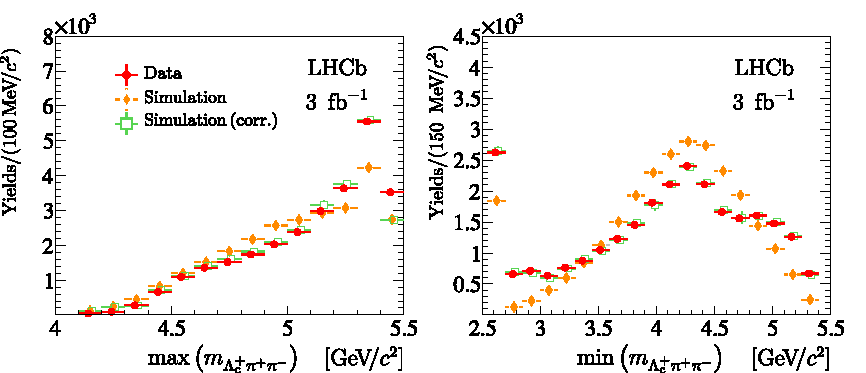
\includegraphics[width=\linewidth]{figures/reweighting-lcpipi}
  %  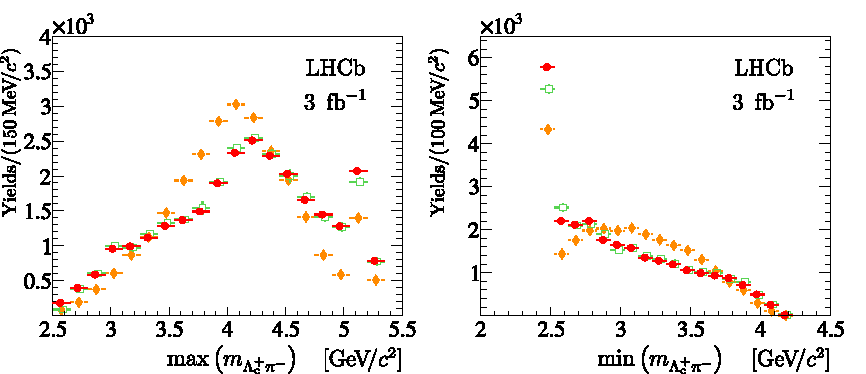
\includegraphics[width=\linewidth]{figures/reweighting-lcpim}
  %} \parbox{.33\linewidth}{
  %  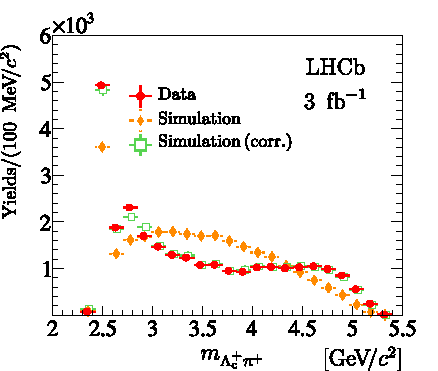
\includegraphics[width=\linewidth]{figures/reweighting-lcpip}
  %}
  \\ \vfill \centering [JHEP 03 (2022) 153]
\end{frame}%}}}

\begin{frame}[label=mva-approach]%{{{
  \frametitle{Отбор событий Run 1 (2011--2012) \& 2 (2015--2018)}

  Предварительный отбор, за которым следует многопеременный анализ:
  \begin{itemize}
    \item 19 входных переменных: кинематика, качество реконструкции 
      и идентификации,
    \item Тренировка только на данных, 9-кратная перекрестная проверка,
  \end{itemize}

  \vfill \centering
  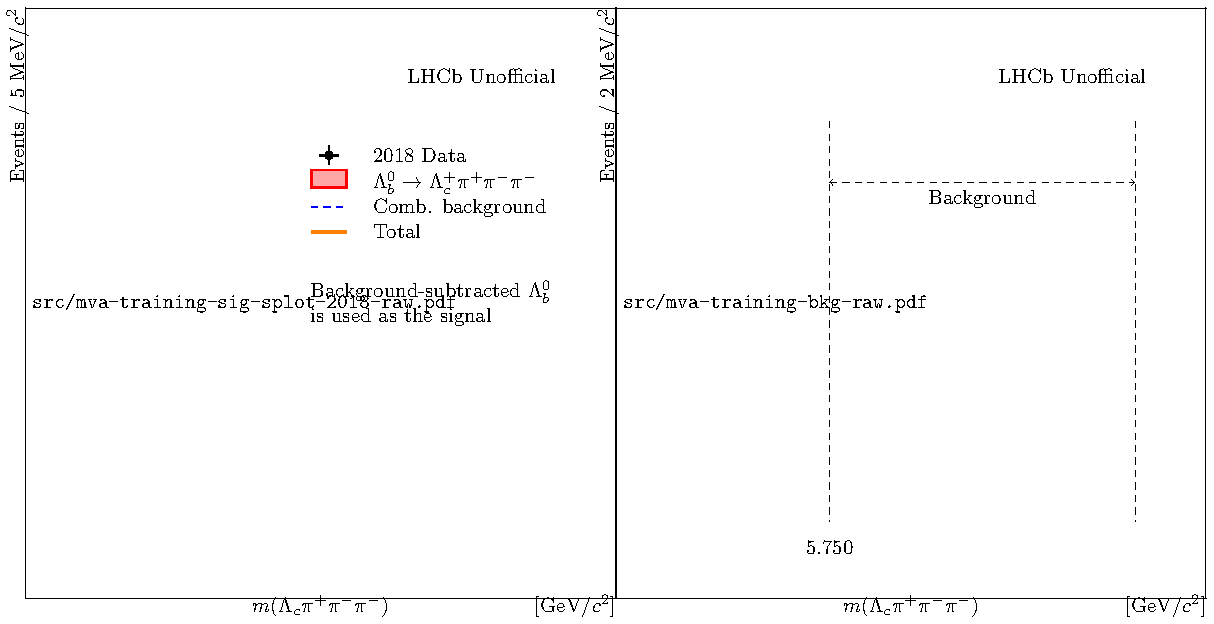
\includegraphics[width=.9\linewidth]{figures/mva-training-sig-bkg}
\end{frame}%}}}

\begin{frame}[label=mva-result]%{{{
  \frametitle{Улучшение качества сигнала в результате MVA}
  \centering
  \begin{tabular}{cc}
    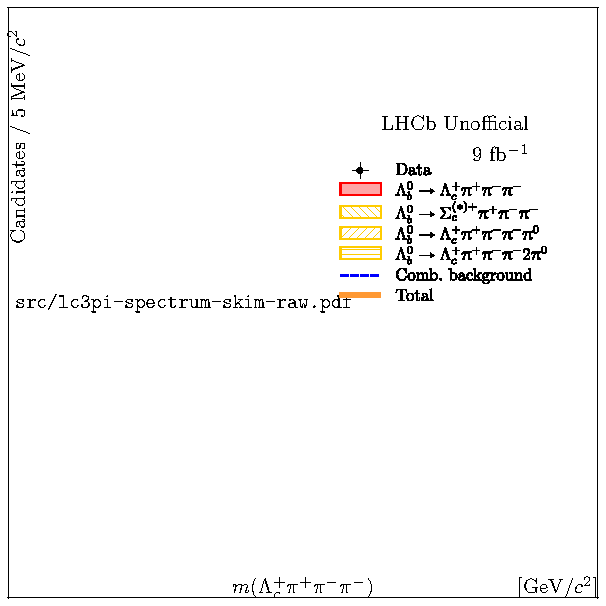
\includegraphics[width=.48\textwidth]{figures/lc3pi-spectrum-skim} &
    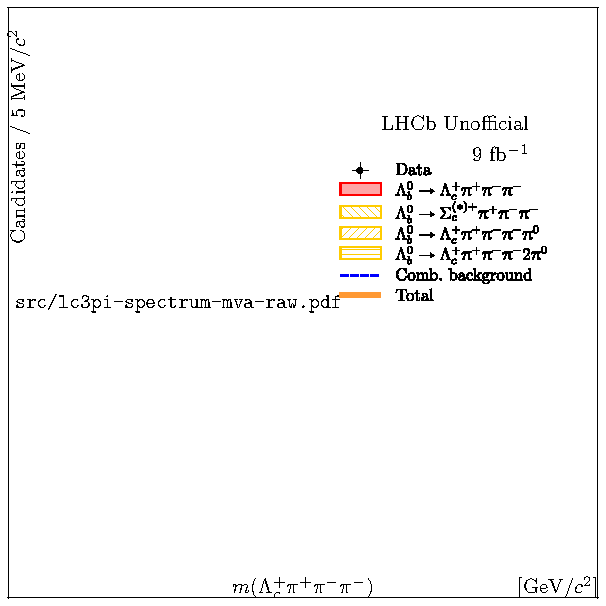
\includegraphics[width=.48\textwidth]{figures/lc3pi-spectrum-mva} \\
    После предварительного отбора &
    После MVA \\
  \end{tabular}
  \vfill
  Сокращение фона в 5 раз при потере лишь 5\% сигнала.
  \begin{tabular}{r@{\hspace*{1ex}}l}
    По~сравнению с~Run~1 сигнал возрос в~24 раза: &
    $\mathbf{3\times}$ от~$\mathcal{L}$ (3~$\to$~9~фб$^{-1}$), \\
    & $\mathbf{8\times}$ от~отбора. \\
  \end{tabular}
  % Уменьшение сигнала на 5\%, а фона -- в 5 раз.
  % \\ Увеличение сигнала в 24 раза по сравнению с Run 1.
  %, а фон -- в 70...
  % Сигнал уменьшился с 650 до 620 на 5\%,
  % Фон уменьшился с 3460 до 630 на 80\%.
  % Run 1: 26k vs 9k
\end{frame}%}}}

\begin{frame}[label=vetoes]%{{{
  \frametitle{Финальный отбор: исключение пикующего фона}
  \centering
  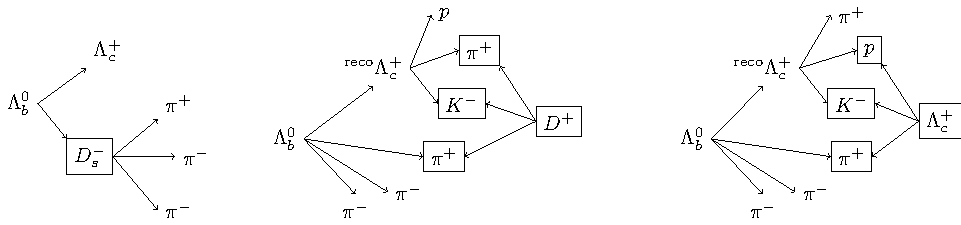
\includegraphics[width=\linewidth]{figures/veto-diagram}
  \\\vfill
  \bottomleft{\rotatebox{90}{[JHEP 03 (2022) 153]}}{
    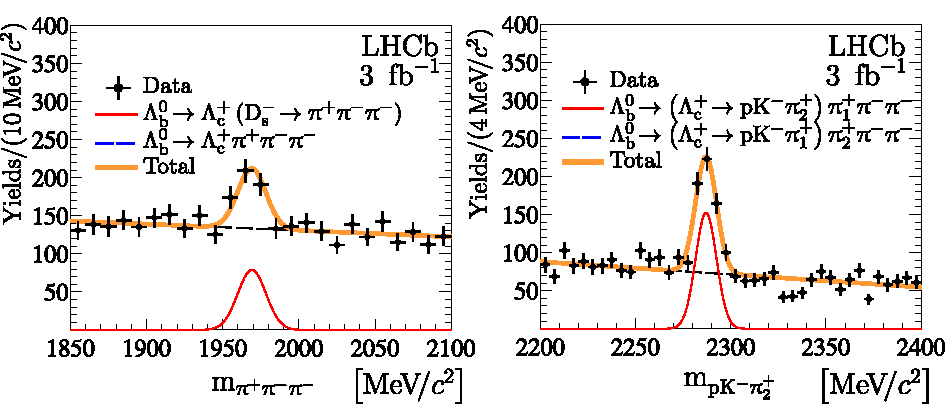
\includegraphics[width=.8\linewidth]{figures/veto-Ds-Lc-fromnote}
  }
\end{frame}%}}}

\begin{frame}[label=conclusion]%{{{
  \frametitle{Итоги}

  \begin{itemize}
    \item На~большой статистике, собранной детектором LHCb в~периоды 
      2011--2012 и~2015--2018, изучается распад $\Lb\to\Lc\pip\pim\pim$.
    \item Распад $\Lb\to\Lc\pip\pim\pim$ имеет богатую резонансную 
      структуру и~поэтому перспективен.
    %\item Распад $\Lb\to\Lc\pip\pim\pim$ имеет богатую резонансную 
    %  структуру и~чрезвычайно большую статистику, собранную детектором 
    %  LHCb, что делает его очень перспективным.
    \item Ожидается существенный вклад в~адронную спектроскопию и~поиск 
      новых состояний.
    \item Ожидается существенное уточнение масс и~естественных ширин 
      очарованных барионных резонансов $\Lcstar$, $\Scstar$.
    \item Работа по~изучению очарованных барионов в~распаде 
      $\Lb\to\Lc\pip\pim\pim$ активно продвигается.
  \end{itemize}
\end{frame}%}}}

\end{document}

Изучение многочастичных распадов прелестного Lb бариона на LHCb
Гусейнов А.-К. Д. 1
1 аспирант
Московский государственный университет имени М.В. Ломоносова, 
физический факультет, Москва, Россия
E–mail: guseynovkerim@gmail.com

Многочастичные безлептонные распады тяжелых барионов широко
востребованы, поскольку служат хорошей проверкой непертурбативных
подходов в квантовой хромодинамике. Так, согласно эффективной теории
тяжелых кварков, тяжелый кварк, масса которого существенно больше
константы КХД, находясь в барионе, образует практически статичное
цветовое поле и связывается с легким дикварком. Подобное рассмотрение
позволяет делать выводы как касательно протекания распадов, так
и касательно адронной спектроскопии.

В то же время, ввиду большого высвобождения энергии при слабых распадах
тяжелых кварков образуется множество адронных резонансов. Мгновенные
распады резонансных состояний приводят к большому числу конечных
продуктов распада, в результате чего многочастичные распады обладают
богатой резонансной структурой.

Детектор LHCb, расположенный на Большом адронном коллайдере в ЦЕРНе,
предоставляет уникальные возможности по изучению распадов тяжелых
- и -адронов. Набор данных протон-протонных соударений, записанный
детектором LHCb на протяжении периодов работы Run 1 и Run 2,
соответствует интегральной светимости . Настолько высокая статистика
позволяет в деталях изучать редкие многочастичные распады, а также
возникающие в них промежуточные резонансы.

В представленной работе уделяется внимание распаду , извлечению спектров
сигнальных событий, а также изучению присутствующих промежуточных
очарованных резонансов, включая, в том числе, уже хорошо изученные
, , , .
